%----------------------------------------------------------------------------------------
%	CHAPITRE 1
%----------------------------------------------------------------------------------------
\chapter{Test logiciel et automatisation} % Nom du premier chapitre

\label{Chapter1} % For referencing the chapter elsewhere, use \ref{Chapter1} 


%----------------------------------------------------------------------------------------
%	SECTION 1
%----------------------------------------------------------------------------------------
\section{Introduction}

%TODO INTRODUCTION
« Tester revient à confronter par des moyens statiques (analyse de code, revue, etc.) ou par des moyens dynamiques (exécution avec des valeurs particulières) les spécifications du logiciel, c’est à dire ce qu’il doit faire et éventuellement sous quelles contraintes (temps, utilisation de la mémoire, etc.), à sa réalisation, c’est à dire de quelle façon il répond au besoin exprimé en enchainant différentes actions élémentaires. »\cite{jfpp-test}

Le test logiciel est une part importante du cycle de développement d'une application et devient vite indispensable pour pérenniser les projets puisqu'elle permet à la fois de s'assurer du comportement d'un logiciel mais aussi de faciliter la maintenance en écartant tous cas de régression lors de l'ajout de nouvelles fonctionnalités ou de simples patchs correctifs.

L'importance de cette activité dépend fortement du domaine de l'application.
Par exemple quand la sécurité des données d'une société, d'un chef d'état ou des vies humaines peuvent être impactés par l'exécution d'un programme comme c'est le cas dans les logiciels embarqués en aéronautique, elle prend une place prépondérante et on ira jusqu'à utiliser des techniques de vérification pour s'assurer à un taux proche de 100\% que l'exécution du logiciel correspond aux spécifications définies. 
Une telle assurance est parfois fondamentale puisque une erreur lors de l'écriture du logiciel peut causer un \textit{bug} majeur et être particulièrement couteuse. Un des cas les plus célèbres est celui-ci associé au programme du décollage de la fusée Ariane 5\cite{ariane5} qui eu pour cause l'explosion de celle ci en plein vol après seulement quelques secondes de décollage. Erreur causée par le plantage du système de guidage inertiel principal à cause d'un simple dépassement d'entier, qui aurait donc pu être corrigé en testant les bornes maximales des entiers.

Cette activité à tout de même de nombreux inconvénients puisqu'elle demande du temps pour être réalisée correctement mais aussi une certaine expertise et est plutôt exigeante intellectuellement. Il ne s'agit pas de tester le programme au hasard en espérant trouver des erreurs mais il faut parfois penser plus loin que le comportement général du programme et donc analyser aussi le comportement des fonctions, des composants et de leurs intégrations avec d'autres logiciels ou d'autres environnements.

Le test logiciel est donc couteux et on lui attribue souvent à lui seul 50\% à 75\% du coût total de développement\cite{software-cost} pour que les logiciels produits soient un minimum fiables. C'est donc impératif pour l'industrie de réduire le coût et d'améliorer son efficacité tout en automatisant son processus. 

Il est aussi indispensable au développement logiciel et c'est une des parties fondamental des disciplines du génie logiciel. Aucune surprise que ce domaine et plus spécifiquement que la génération automatique de tests est fait l'objet d'autant de recherche ces dernières années et de nombreux outils et techniques ont émergés\cite{orchestrated-survey-automated-test}.
En même temps, les logiciels se sont complexifiés pour tenir compte des nouvelles techniques de programmation facilitant le développement, la maintenance, les modifications mais aussi devant supporter le bagage informatique des années précédentes. Cette hétérogénéité peut devenir problématique, puisque les programmes peuvent avoir des supports différents, que ce soit le \textit{smartphone}, l'ordinateur de bureau, les consoles de jeux ou même les objets connectés (\textit{IOT}: Internet Of Things) qui peuvent interagir avec l'environnement physique tout en communicant avec d'autres machines sur le réseau.

%----------------------------------------------------------------------------------------
%	SECTION 2
%----------------------------------------------------------------------------------------
\section{Génération de tests}
La génération automatique de tests\cite{orchestrated-survey-automated-test} est un domaine déjà bien développé qui permet aujourd'hui grâce à différentes analyses à partir du code comme celle de l'arbre syntaxique abstrait, du graphe de flot de contrôle (CFG) et d'application de méthodes comme l'exécution symbolique, concolique ou de model-checking, d'extraire des propriétés parfois abstraites du code pour identifier des jeux de tests pertinent pour s'assurer de la qualité du programme\cite{EFSM}.
Deux analyses majeures sont utilisées qui sont l'analyse statique, qui couvrent les méthodes permettant d'obtenir des informations d'un programme à partir de son code source sans l'exécuter et l'analyse dynamique qui couvrent les méthodes utilisées pour observer le comportement d'un programme à l'exécution.

\subsection{Exécution symbolique}

\subsubsection*{Définitions}
L'exécution symbolique\cite{symbolic-execution-by-king} est une technique de type boîte blanche (on peut observer la structure interne du programme) qui permet d'analyser le comportement d'un programme en remplaçant les données par des symboles. 
Au lieu d'exécuter le programme et de suivre l'évolution des valeurs des variables concrètes en mémoire et comment elles influent sur le comportement du programme, on construit un arbre des chemins d'exécutions possibles à partir de valeurs symboliques en entrée et des contraintes récoltées sur les différents chemins.
Au final, les valeurs de sorties calculées par le programme seront exprimées comme fonction des valeurs symboliques d'entrée.

Dans le domaine du test logiciel, l'exécution symbolique est utilisée pour générer des jeux de tests pour couvrir les branches d'exécutions possibles du programme ou pour s'assurer que certains chemins d'exécutions sont irréalisables sous certaines conditions.
Un chemin d'exécution possible (exemple figure: \ref{symbolic-execution-example1}) est une séquence de condition qui sont soit « vraie » soit « fausse » exprimée en fonction des contraintes d'entrées et celles récoltées tout au long du chemin. Tous les chemins d'exécution du programme peuvent être représentés en utilisant une structure d'arbre.

On appelle la contrainte de chemin (Path constraint: PC) une formule booléenne qui représente l'équation de toutes les contraintes que doivent assurer les valeurs symboliques d'entrées pour suivre un chemin d'exécution. Par exemple, la figure \ref{symbolic-execution-example1} montre en bas à gauche un exemple de contrainte de chemin ($[PC]: x < 0 \bigwedge x > -10$) signifiant que la variable symbolique $x$ en entrée doit satisfaire ces contraintes pour suivre ce chemin d'exécution et on peut donc voir que chaque chemin d'exécution possède ses propres contraintes.\\

% Exemple exécution symbolique
\begin{center}
    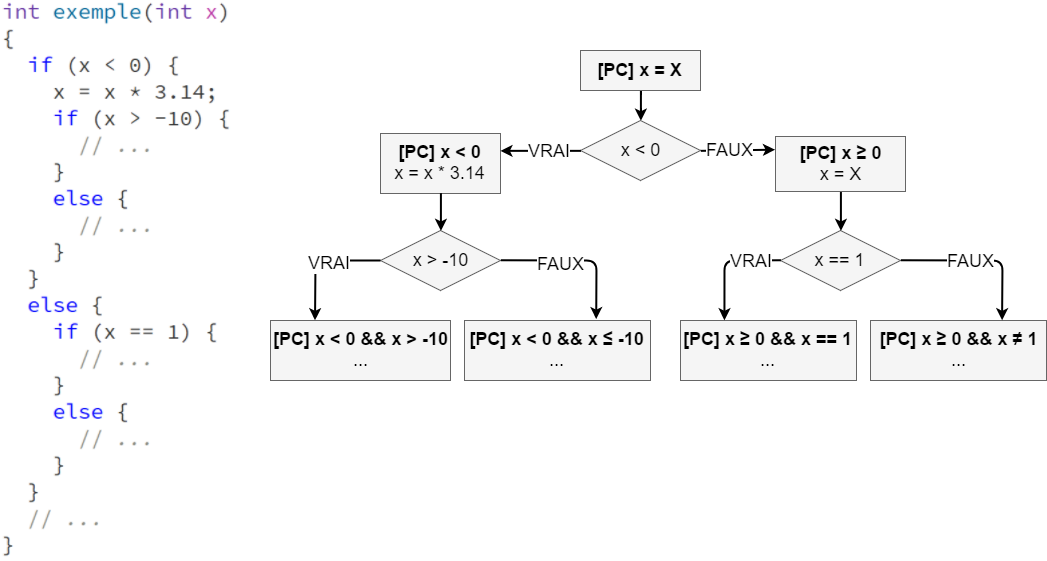
\includegraphics[scale=0.4]{../ressources/images/dynamic_execution_example.png}
    \captionof{figure}{Exemple des chemins d'exécutions possibles récoltés grâce à l'exécution symbolique d'un programme C.}
    \label{symbolic-execution-example1}
\end{center}

%TODO 
%C'est donc une technique qui tire partir des bénéfices des méthodes d'analyses statiques ainsi que des méthodes dynamiques.
%Le problème des méthodes statiques sont les faux positifs et que le programme l'analyse peut potentiellement s'éloigné beaucoup de l'exécution réel du programme.

\subsubsection*{Limitations}
Bien que la technique d'exécution symbolique a été proposée dans les années 70\cite{symbolic-execution-by-king}, cette technique n'a reçu l'attention des chercheurs que récemment pour deux raisons. 
Premièrement l'application de l'exécution symbolique sur des programmes conséquents en application réelle requiert de résoudre des équations complexes avec beaucoup de contraintes. C'est là où les récentes avancées des solveurs de contraintes ont été bénéfiques. Un solveur de contrainte permet de résoudre des équations de satisfaction de contraintes. Il est donc capable d'évaluer la faisabilité d'un ensemble de contraintes donné et permet donc de déterminer si un chemin donné par l'exécution symbolique est faisable ou non. Ces outils sont donc utiliser conjointement à l'exécution symbolique pour limiter l'exécution sur les chemins atteignables.
Deuxièmement, l'exécution symbolique est une technique extrêmement couteuse en ressource, bien plus que les méthodes classiques d'analyse statique. Ce coût est associé à la multiplicité des chemins d'exécution possibles dans des programmes complexes et à la complexité des contraintes des chemins qui augmentent au fur et à mesure du parcours. Heureusement, les puissances de calculs actuelles ont largement augmentées et permettent de réaliser cette analyse dans certaine condition.

Même si l'exécution symbolique semble être théoriquement capable d'analyser en profondeur le comportement d'un programme, cette technique souffre encore de problèmes majeurs quand elle est confronté à de réels programmes:\\
\begin{itemize}
\item Le premier est l'explosion des chemins, c'est à dire que le nombre de chemins d'exécutions possible évolue exponentiellement. Il est donc impératif de trouver des méthodes pour réduire le nombre de chemins à évaluer.\\
\item Le deuxième est la divergence de chemins où \textit{path divergences}. On parle de chemin divergent quand le comportement analysé par l'exécution symbolique est différent du comportement concret à l'exécution. Un tel cas peut arriver plus fréquemment qu'on ne le pense puisque les programmes s'exécutent sur des environnement complexes communicant avec plusieurs composants. L'exécution symbolique ne fait qu'isoler le comportement du programme et il est difficile de tenir compte de tous les éléments pouvant affecter le comportement du programme.\\
\item Le troisième est la complexité des contraintes qui peuvent parfois être trop importantes pour être résolu par un solveur de contraintes. Des contraintes impliquant des opérations de multiplication et de division ou d'autres opérations non linéaires ont tendances à faire rapidement exploser la complexité des contraintes. Si les contraintes de chemins sont indécidables, alors les chemins possiblement couverts par l'exécution symbolique sont limités.

\end{itemize}

%TODO Techniques pour résoudre les problématiques posées plus haut
\subsubsection*{Techniques pour contourner les limitations}
Bien que ces problématiques limitent fortement l'utilisation des techniques d'exécution symbolique sur de réelles applications, il existe des méthodes qui permettent en partie de contourner ces limitations. 
Par exemple, pour contourner le problème d'explosion des chemins, des techniques permettent de guider l'exploration en ce limitant aux chemins amenant à un certain objectif, par exemple celui de couvrir une portion du programme.
Pour limiter la complexité grandissante des contraintes du problème, il est possible de joindre l'exécution symbolique du programme à son exécution concrète, c'est l'exécution concolique. Dans ce cas de figure, le programme est exécuté sur des valeurs concrètes ainsi que sur des valeurs symboliques ce qui permet, si des contraintes deviennent trop complexes, de les simplifier en utilisant les valeurs concrètes du programme. Au final, on se sert de l'exécution du programme pour construire les chemins d'exécutions et de l'exécution symbolique pour limiter le nombre de chemins à exécuter réellement.
%Nous ne souhaitons pas présenter toutes ces méthodes de manière exhaustive puisqu'elles sont nombreuses\cite{orchestrated-survey-automated-test} et certaines de s'appliquent qu'à des cas spécifiques donc nous présenterons une technique pour l'explosion des chemins et une pour la complexité des contraintes. 

\subsection{Model-Based Testing}

\subsubsection*{Définitions}
Model-Based Testing (MBT) est une méthode semi formelle qui utilise des modèles du système testé (\textit{System Under Test: SUT}) pour générer des cas de tests.
Les modèles peuvent représenter des abstractions du comportement du SUT et ils pourront être utilisés pour comparer le comportement théorique modélisé au comportement réel du SUT.
De manière générale, le SUT est modélisé comme une boite noire, c'est à dire que son comportement interne n'est pas analysé. Les modèles décrivent alors des séquences d'entrées et de sorties possibles.
Un des gros avantages de ce type de méthode est qu'elle permet d'abstraire le comportement souhaité du logiciel du code et un modèle pourrait donc définir le comportement souhaité d'un programme, qu'il soit écrit en C ou en Java par exemple.

%Model-based testing (MBT) est une méthode de modélisation semi-formelle dans l'objectif de concevoir de manière automatique ou non des cas de tests. Les modèles peuvent être utilisés pour représenter le comportement voulu du système testé puis pour établir une stratégie de test à partir des modèles.
%
%pour représenter le comportement souhaité du système, pour représenter la stratégie de tests 
%
%est une approche de type ? boîte noire ? c'est
%à dire basée sur la représentation d'un programme sans considérer son fonc-
%tionnement interne. Cette approche vise à identi?er les comportements de
%l'application ou de composants pour véri?er leur comportement en fonction
%des paramètres d'entrées/sorties possibles.
%L'objectif est de trouver un ensemble de valeurs d'entrées pour su?samment tester le comportement du
%programme ou d'une fonctionnalité (couverture de test) à partir, par exemple
%de spéci?cation algébrique [3].

\subsubsection*{Limitations}
Dans notre démarche, nous souhaitons comparer le comportement de programmes dont l'exécution devrait être identique. Nous avons donc une approche qui est orientée à partir du code, c'est à dire que l'objectif des programmes dépend du code source de la programmation qui décrit le comportement souhaité. 
Dans une approche à partir de modèle, l'objectif est souvent inverse. Il est plus facile de décrire les modèles et ensuite de générer une partie du code et des tests. 
Si nous avions décidé d'écrire les exercices de programmation sous forme de modèles, nous aurions pu estimer plus facilement les bénéfices d'une méthode de modélisation. Nous savions qu'une telle approche nécessiterait une compétence technique supplémentaire de l'évaluateur qui devrait être en mesure de décrire le comportement du programme souhaité sous forme de modèle et c'est pour cela que cette méthode n'a pas été privilégiée.
De plus, la quantité d'informations modélisée est souvent limité puisqu'il s'agit de définir principalement le comportement attendu en fonctions des entrées et des sorties. Avec une approche boîte blanche, nous pouvons observer le comportement interne d'un programme et potentiellement découvrir des éléments internes qui favorise l'émergence d'une divergence de comportements entre deux programmes.

%\subsection{Méthodes aléatoires}
%%TODO Y a t-il d'autres méthodes ?
%La génération de test de manière aléatoire est surement une des méthodes
%les plus évidentes et les plus faciles à mettre en place. Dans certains cas, c'est
%l'unique méthode envisageable si la documentation d'un programme est in-
%complète et que le code source n'est pas accessible. Cette technique a bien sur
%un coup important, l'ensemble des valeurs possibles pour les valeurs d'entrées
%d'un programme est souvent trop complexe. Pour cela, des méthodes de gé-
%nération adaptives sont utilisées. Des méthodes empiriques ont montrées que
%des valeurs d'entrées générant des erreurs ont tendance à former des régions
%contingentes d'erreurs. Il en est inversement de même pour des valeurs d'en-
%trées ne générant aucune erreur [2]. Il s'agit donc de dé?nir des stratégies de
%génération pour couvrir de manière e?cace l'ensemble des valeurs possibles
%en maximisant les chances de tomber sur une valeur d'erreur pour ensuite
%tester les valeurs contingentes.

\subsection{Search-Based Testing}
%TODO Search based testing

\subsubsection*{Définitions}
\textit{Search-based software testing}\cite{search-based-testing} est un sous domaine de \textit{Search-based software engineering}\cite{search-based-software-engineering} qui regroupe l'application des heuristiques de recherche pour résoudre des problèmes du génie logiciel.
\textit{Search-based testing}, lui, est le domaine qui regroupe les techniques de recherche heuristique à des fins de générations de tests. Pour cela, il s'agit de transformer le problème de génération de tests en un problème d'optimisation qui peut être résolu avec ces techniques.

Les techniques de recherche heuristiques sont des alternatives pour attaquer les problèmes où l'espace de recherche est trop important. Cette situation est fréquemment rencontrée lorsqu'il s'agit d'établir l'ensemble des chemins d'exécutions possibles d'un programme pour déterminer des jeux de tests pertinents.
L'objectif n'est donc pas de couvrir toutes les branches possibles, mais de définir une fonction objectif qui guidera automatiquement la recherche pour atteindre un but fixé le plus rapidement possible. C'est d'ailleurs le point crucial de cette méthode, puisque c'est cette fonction objectif qui permettra à l'algorithme de déterminer de bonnes solutions dans un temps raisonnable.
Elle peut donc se montrer efficace pour générer des jeux de tests pertinents et pour optimiser le processus de génération de tests.

La forme la plus simple d'un algorithme d'optimisation - bien que très peu efficace - est une recherche aléatoire. Ici, les jeux de tests sont générés aléatoirement jusqu'à ce que l'objectif soit atteint. Un exemple d'objectif simple peut être le pourcentage de couverture du programme à atteindre. Malheureusement cette méthode est très limitée puisque plus l'espace des valeurs possibles est grand moins les valeurs générées aléatoirement auront une chance d'être suffisamment pertinentes.

D'autres techniques sont plus fréquemment utilisées comme celle du \textit{Hill Climbing} qui, appliquée à l'exécution symbolique, favorise la sélection d'optimum locaux. L'algorithme favorise lors de son parcours les chemins les plus prometteurs, c'est à dire que depuis chaque branchement de l'exécution, il sélectionnera le chemin le plus prometteur (par exemple se rapprochant le plus de la solution). Comme un chapitre entier est réservé aux heuristiques, nous ne décrirons pas plus en détail les méthodes de parcours utilisées puisqu'elles sont quasiment identiques.

\begin{center}
    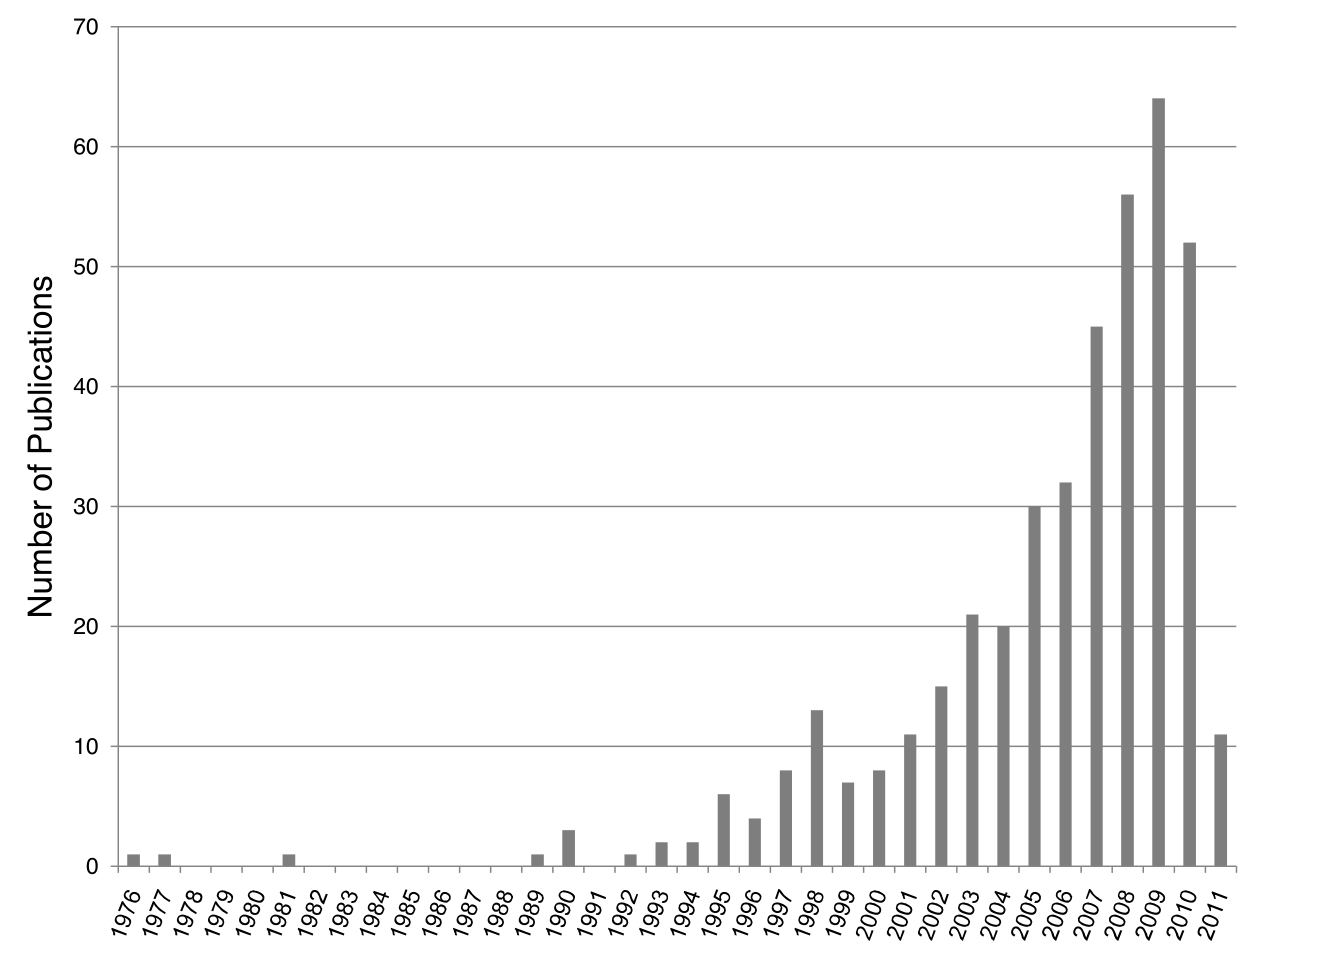
\includegraphics[scale=0.35]{../ressources/images/publications_search_based_testing.png}
    \captionof{figure}{Publications dans le domaine du \textit{Search-Based Software Testing} - source: \textit{Search-Based Software Testing: Past, Present and Future}\cite{search-based-testing}}
    \label{popularity-search-based-testing}
\end{center}


\subsubsection*{Limitations}
Le succès de ces méthodes dépend majoritairement de la qualité de la fonction objectif fixée qui doit permettre de satisfaire un ensemble de critères comme par exemple un pourcentage de couverture des branches à atteindre. De plus, il faut aussi que les outils disponibles puissent tenir compte des critères sélectionnés (le critère peut être indéterminable statiquement ou dynamiquement sur une portion de code) et que l'évaluation de ces critères lors de l'analyse ne soit pas trop longue.

Une fois l'objectif défini, il existe de nombreuses heuristiques de recherche possibles à appliquer. Il faut donc sélectionner la bonne méthode de recherche qui soit apporte un résultat de meilleure qualité, soit le fait en un temps plus raisonnable ou bien les deux à la fois.
Au final, tout le succès de ces méthodes dépend de définition de la fonction objectif qui doit avoir des critères adéquats et déterminables selon la méthode utilisée mais aussi d'une recherche heuristique adaptée au problème qui fasse un compromis entre la qualité de la solution obtenue et le temps d'exécution.

C'est d'ailleurs une limitation importante de ces techniques de recherche puisqu'elles ne sont majoritairement appliquées que pour générer des jeux de tests pour couvrir la plus grand portion du code possible (ou des régions particulière du code ) sans se soucier du comportement de l'application à tester en fonction des valeurs d'entrées.
Heureusement, les méthodes heuristiques permettent d'adapter l'objectif pour qu'il soit pluriel. A l'avenir les défis sont donc de définir des objectifs qui tiennent comptent de multi-critères qui sont déterminables lors de l'analyse et qui permettent de tenir compte du comportement de l'application pour générer des jeux de tests de qualité.

%----------------------------------------------------------------------------------------
%	SECTION 3
%----------------------------------------------------------------------------------------
\section{Détection de divergences entre versions d'un logiciel}

\subsection{Méthode utilisée}
Pour la détection de divergences de comportements entre deux versions d'un même logiciel, il existe des solutions qui permettent de limiter la combinatoire et notamment pour l'exécution symbolique.
Une de ces méthodes proposées est présentée dans l'article \textit{Shadow of a doubt: Testing for divergences Between Software Versions}\cite{shadow} (en référence au célèbre film Alfred Hitchcock: \textit{L'ombre d'un doute}). 

Le postulat de départ est qu'il serait moins coûteux de comparer deux versions d'un même logiciel uniquement aux endroits où le code à été modifié. Au lieu de se baser sur l'analyse complète des deux arbres d'exécution symbolique du programme, nous partirions donc des sous-arbres de ces ensembles, là ou la divergence de code est présente, pour établir l'analyse.
Pour cela, il est proposé de fondre les deux versions du programme en tenant compte des modifications effectuées et ceci grâce à quelques annotations qui permettent de générer des branches d'exécutions séparées là où le code diverge.

%Shadow exemple
\begin{center}
    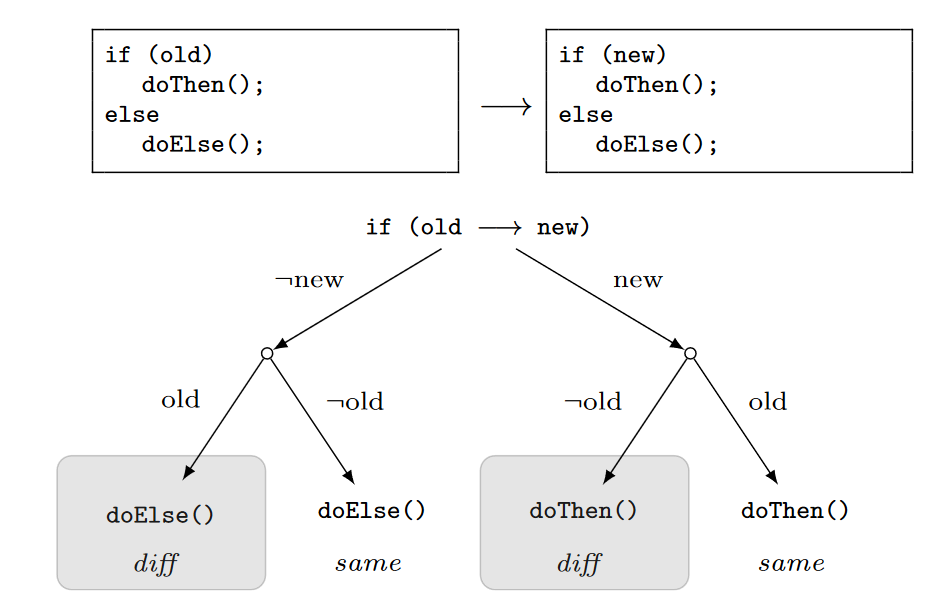
\includegraphics[scale=0.45]{../ressources/images/shadow_example.png}
    \captionof{figure}{Exemple d'un branchemement de l'exécution symbolique tenant compte de la nouvelle version du programme - source: \textit{Article shadow\cite{shadow}}}
    \label{shadow-example}
\end{center}


\subsection{Limitations}
%TODO Il faut le coder, actuellement cette méthode n'est pas automatisée

%Limitation dans notre cas à nous
Même si cette approche paraît particulièrement intéressante, nous doutons de son intérêt dans notre cas où nous ne disposons pas de deux versions d'un même programme mais de n programmes implémentant tous une même spécification (description en langue naturel ou par des formules mathématiques de ce qui doit être produit). 
Potentiellement, ces programmes pourraient être intégralement différents dans leur structure bien que leurs comportements à l'exécution seraient identiques. Il est donc plus difficile de bénéficier de la proximité des programmes pour limiter la combinatoire de l'exécution symbolique.\\

{\setlength{\parindent}{0cm}\textbf{Conclusions:}}

Les approches que nous avons vu précédemment sont souvent limitées\cite{test-auto-solved-yet} de par la complexité grandissante des programmes qui confrontent ces méthodes à l'explosion du nombre de chemins, du nombre d'états ou de contraintes possibles. Pour représenter ces états et chemins, ces méthodes reposent sur des modèles d'arbres qui ne peuvent être parcourus en intégralité à cause de leur taille. Les algorithmes de parcours actuellement utilisés reposent majoritairement sur des stratégies simples comme le parcours en profondeur qui est connu pour être particulièrement couteux mais qui a le bénéfice de trouver au moins un chemin d'exécution possible.

Ces dernières années, grâce à la maturation des recherches sur les différentes stratégies et heuristiques de parcours de graphe (notamment celles avec apprentissage) et des applications récentes sur des problèmes concrets, comme celui du jeu de go où l'ordinateur \textit{AlphaGo}\cite{AlphaGo-research} qui grâce à une implémentation de l'heuristique du Monte Carlo Tree Search a réussi à battre le champion du monde actuel, ces méthodes ce sont popularisées.

C'est pourquoi, nous pensons que des méthodes de Search-based Testing combiner à des méthodes d'exécution symboliques pourraient permettre de contourner nos contraintes. Nous espérons pouvoir utiliser ou simplement nous inspirer des heuristiques avec apprentissages pour diminuer l'espace de recherche plus nous analysons de programme.

